\documentclass{standalone}
	\usepackage{tikz}
		\graphicspath{ {figures/AM_11_431/} }
	\begin{document}
\begin{tikzpicture}[node distance=0.01cm and 3cm]
 \node[anchor=center] (0) at (0,-0.8) { 11 \ (block5\_conv1) };
\node[anchor=center] at (6,-0.8) { 12 \ (block5\_conv2) };
 \foreach \label [count=\i] in {L10_F23.png,L10_F42.png,L10_F430.png,L10_F334.png,L10_F483.png,L10_F465.png,L10_F209.png,L10_F88.png,L10_F463.png,L10_F410.png} { 
 
	\node[draw=none] (\i) at (0,-\i*6em) {\includegraphics[width=0.3\textwidth]{\label} }; 
  }
\node[] (R) at (6,-5.5*6em) {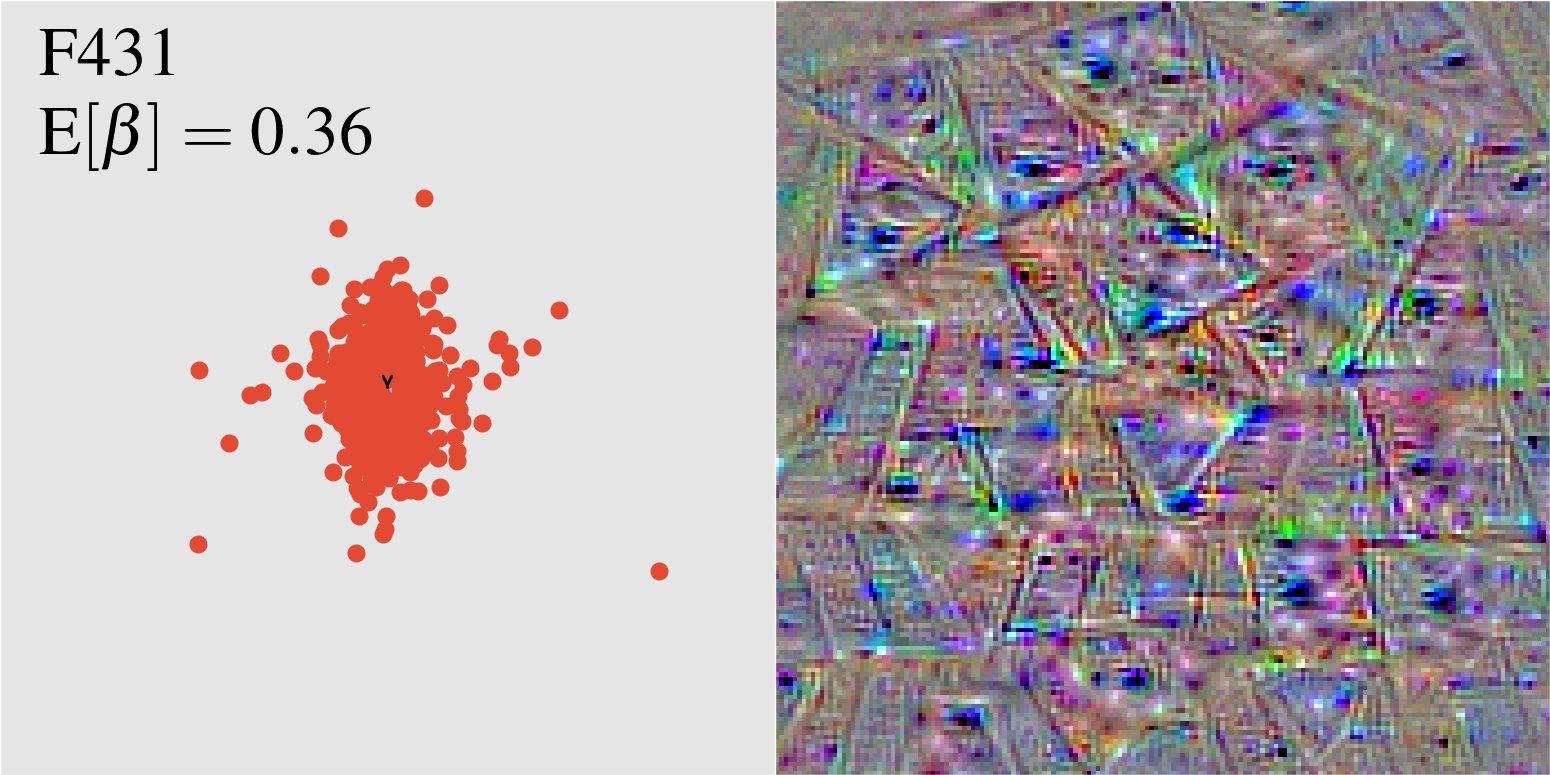
\includegraphics[width=0.3\textwidth]{ L11_F431.png } }; % Adjust the y-coordinate to center
 \draw (1.east) -- (R) node[pos=0.5, circle, draw, fill=white, minimum size=8pt, inner sep=0pt, scale=0.5] { 1.0 }; 
 \draw (2.east) -- (R) node[pos=0.5, circle, draw, fill=white, minimum size=8pt, inner sep=0pt, scale=0.8] {$-$}; 
 \draw (3.east) -- (R) node[pos=0.5, circle, draw, fill=white, minimum size=8pt, inner sep=0pt, scale=0.5] { 1.0 }; 
 \draw (4.east) -- (R) node[pos=0.5, circle, draw, fill=white, minimum size=8pt, inner sep=0pt, scale=0.8] {$-$}; 
 \draw (5.east) -- (R) node[pos=0.5, circle, draw, fill=white, minimum size=8pt, inner sep=0pt, scale=0.8] {$+$}; 
 \draw (6.east) -- (R) node[pos=0.5, circle, draw, fill=white, minimum size=8pt, inner sep=0pt, scale=0.8] {$-$}; 
 \draw (7.east) -- (R) node[pos=0.5, circle, draw, fill=white, minimum size=8pt, inner sep=0pt, scale=0.8] {$+$}; 
 \draw (8.east) -- (R) node[pos=0.5, circle, draw, fill=white, minimum size=8pt, inner sep=0pt, scale=0.8] {$-$}; 
 \draw (9.east) -- (R) node[pos=0.5, circle, draw, fill=white, minimum size=8pt, inner sep=0pt, scale=0.8] {$+$}; 
 \draw (10.east) -- (R) node[pos=0.5, circle, draw, fill=white, minimum size=8pt, inner sep=0pt, scale=0.8] {$+$}; 
\end{tikzpicture}
\end{document}
